\section{Projecten}

Binnen \customerdomain is er de mogelijkheid om projecten aan te maken. Projecten zijn technisch gezien \emph{subsites}. Deze kunnen worden beheerd op \emph{Structuur} $\rightarrow$ \emph{Dominion} of direct op \drupalpath{admin/structure/dominion}.

\subsection{Project toevoegen}\label{projecttoevoegen}

Klik in het subsites overzicht op \emph{Add project subsite} of ga direct naar \\ \drupalpath{admin/structure/dominion/add/project}. In het formulier moeten de volgende gegevens worden ingevuld:
\begin{itemize}
\item Naam: naam van de subsite (bijv. "Hanzelijn")
\item Domain type: klik op \emph{Use a directory}
\item Directory: vul het pad van de subsite in (bijv. "projecten/hanzelijn")
\end{itemize}
De laatste optie is alleen zichtbaar wanneer \emph{directory} als \emph{domain type} is opgegeven. Binnen de Prorail site is het de conventie om het pad te beginnen met "projecten/". Het wordt tevens aanbevolen om enkel kleine letters te gebruiken aangezien het pad hoofdlettergevoelig is en hoofdletters in URL's niet gangbaar zijn.

Op het ingevoerde pad zal de subsite zichtbaar worden. Hierop is ook de projectnode te zien aangezien dat de voorpagina is van de subsite. De node zelf heeft daarom geen alias.

\subsection{Project wijzigen}

Waar een wijziging voor een project doorgevoerd moet worden is afhankelijk van de aard van de wijziging. Kortweg:
\begin{itemize}
\item Naam van subsite
\begin{itemize}
\item In de titelbalk $\rightarrow$ dominion
\item Titel op de voorpagina en naam op kaart $\rightarrow$ bewerk project node
\item Naam op menu-item naar voorpagina $\rightarrow$ bewerk menu-item
\end{itemize}
\item Pad van subsite $\rightarrow$ dominion
\item Tekst van de voorpagina $\rightarrow$ bewerk project node
\item Weergave op de kaart $\rightarrow$ bewerk project node
\end{itemize}
De naam van de subsite komt op die plaatsen terug. Bij het aanmaken van een nieuwe projectsubsite worden deze alle 3 automatisch gezet. Bij het wijzigen worden de wijzigingen echter niet automatisch doorgevoerd.

\subsection{Redacteuren}

Na het aanmaken van het project kunnen redacteuren worden toegevoegd. Klik hiervoor in de lijst met subsites op de link \emph{redacteuren}. Er komt nu een lijst van de redacteuren die reeds gekoppeld zijn aan deze subsite. Klik op \emph{redacteur toevoegen} om een bestaande gebruiker toe te voegen als redacteur voor deze subsite. Het is niet mogelijk om hier nieuwe gebruikers aan te maken, dus de gebruiker moet reeds geregistreerd zijn. In deze pagina kunnen bestaande gebruikers toegevoegd worden op basis van het e-mailadres of gebruikersnaam. Hier kunnen ook gebruikersrollen worden toegevoegd. Het is hier enkel mogelijk om rollen toe te voegen. Rollen die niet aangevinkt zijn worden dus niet ontnomen.

\subsection{Inhoud beheren}

Het beheren van inhoud binnen de project subsite werkt hetzelfde als voor doelgroepen. Bij het aanmaken en bewerken van content zijn de projecten zichtbaar onder \emph{Contentdeling}. Tevens kan in de \emph{Workbench} het project worden gevonden onder het filter \emph{Subsite}.

\subsection{Menu}

Elk project krijgt een eigen menu dat zichtbaar is als blokje in de rechterkolom. Eindredacteuren en redacteuren van deze subsite zullen het menu te zien krijgen in het menu beheer\seeone{menu}.

Pagina's die onder een project worden toegevoegd komen \emph{niet} automatisch in het menu. Dit zal dus altijd handmatig gedaan moeten worden.

\subsection{Toegangsrechten}

Het is mogelijk om een project subsite af te schermen van het publiek en alleen toegankelijk te maken voor redacteuren. Klik hiervoor bij het toevoegen of bewerkern van een (project) subsite op \emph{Access permissions}.

\begin{center}
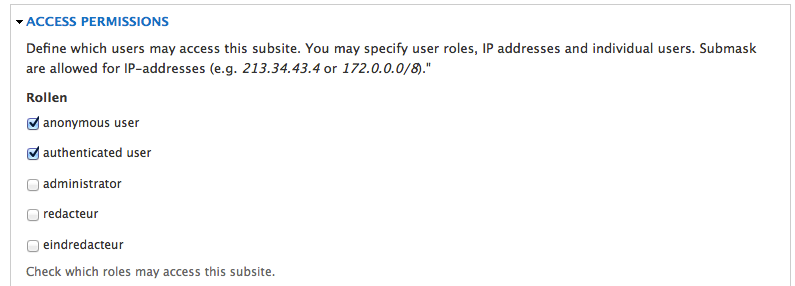
\includegraphics[width=\textwidth]{img/dominionaccess.png}
\end{center}

Hier kan worden aangevinkt welke gebruikersrollen toegang hebben tot deze subsite. Standaard staan "anonymous user" en "authenticated user" aan. Dit zijn respectieveliljk alle niet-ingelogde en alle ingelogde bezoekers en komt samen dus neer op alle bezoekers. Door deze uit te vinken en alleen de redacteurrollen aan te vinken zal deze subsite alleen toegankelijk worden voor redacteuren.




